\documentclass{article}
\usepackage{parskip}
\usepackage{graphicx}
\usepackage[backend=biber, style=alphabetic]{biblatex}
\usepackage{listings}
\usepackage{hyperref} % must be last import

\addbibresource{procesrapport.bib}

\newcommand{\projectname}{Decentraliseret dataudveksling i notesapplikation}
\newcommand{\student}{Marcus Haukelid Larsen}
\newcommand{\supervisor}{?}

\begin{document}

\pdfbookmark[1]{Forside}{frontpage}

\begin{center}
  {\Huge \textbf{\projectname}}

  \vspace*{\fill}

  {\Large \textbf{\student}}

  \vspace*{\fill}

  {\large \textbf{Procesrapport}}
\end{center}

\thispagestyle{empty}

\newpage
\begin{center}  
  {\large \textbf{Elev:} \student}
  \vspace*{\fill}

  {\large \textbf{Projektnavn:} \projectname}
  \vspace*{\fill}

  {\large \textbf{Uddannelsessted:} Techcollege, Struervej 70, 9220 Aalborg Øst, Denmark}
  \vspace*{\fill}

  {\large \textbf{Elevplads:} RTX A/S, Strømmen 6, 9400 Nørresundby, Denmark}
  \vspace*{\fill}

  {\large \textbf{Projektperiode:} 05/02-2026 - 17/03-2026}
  \vspace*{\fill}

  {\large \textbf{Afleveringsdato:} 17/03-2026}
  \vspace*{\fill}

  {\large \textbf{Fremlæggelsesdato:} 20 el. 23/03-2026}
  \vspace*{\fill}

  {\large \textbf{Vejleder:} \supervisor}
  \vspace*{\fill}

  {\large \textbf{Underskrift:}}
  \vspace*{\fill}
  
  \begin{tabular}{p{6cm} p{6cm}}
    \hrulefill & \hrulefill \\
    Vejleder (\supervisor) & Elev (\student)
  \end{tabular}
\end{center}

\thispagestyle{empty}

\newpage
\tableofcontents

\newpage

\section{Læsevejledning}
Denne rapport er struktureret, så læseren først får en introduktion til
projektets kontekst. I indledningen præsenteres baggrunden for casen
og de centrale spørgsmål, som rapporten søger at besvare.

Efter indledningen følger en beskrivelse af projektplanlægningen, hvor
arbejdsprocessen og tidsplanen præsenteres.
Metodologiafsnittet forklarer, hvordan projektet er gennemført, og er
opdelt i tre underafsnit: Brugergrænseflade, Databehandling og Datalagring.

Rapporten afsluttes med en diskussion af projektets begrænsninger samt en
konklusion, som opsummerer de væsentligste resultater og erfaringer.

\section{Indledning}
Vi lever i en digitaliseret verden, hvor ejerskab i stigende grad erstattes af
midlertidig adgang.

Som følge af magtkoncentration er der opstået flere organiserede bevægelser, der
fremhæver decentraliseret digital infrastruktur som et muligt alternativ.

Decentralisering rejser nye politiske spørgsmål om ansvar, regulering og ulighed.
Fraværet af centrale aktører kan vanskeliggøre både kontrol og retlig beskyttelse.

Rapporten beskriver, hvordan produktet er udarbejdet, hvilke delelementer det
indebærer, og hvilke begrænsninger der er identificeret undervejs.

\section{Casebeskrivelse}
Vi lever i en digitaliseret verden, hvor ejerskab i stigende grad
erstattes af midlertidig adgang. Denne udvikling rejser politiske
spørgsmål om magt, rettigheder og afhængighed i relationen mellem
borgere, stater og globale tech-giganter. Når data fungerer som den
centrale valuta i den digitale økonomi, forskydes magten fra borgeren
til de platforme, der kontrollerer indsamling, behandling og
anvendelse af disse data.

Som reaktion på denne magtkoncentration er der opstået flere
organiserede bevægelser, som fremhæver decentraliseret digital
infrastruktur som et muligt alternativ. I en decentraliseret model
er data og digitale aktiver ikke samlet hos enkelte platforme, men
distribueret på tværs af netværk, hvor brugerne i højere grad 
har kontrol over egne oplysninger og digitale ressourcer.

Decentralisering rejser dog også nye politiske spørgsmål om ansvar,
regulering og ulighed. Fraværet af centrale aktører kan vanskeliggøre
både demokratisk kontrol og retlig beskyttelse, hvilket udfordrer
statens traditionelle rolle som garant for borgernes rettigheder.

\section{Problemformulering}
Hvordan kan decentraliseret dataudveksling i en notesapplikation
bidrage til øget digitalt ejerskab og reducere brugerens afhængighed af
centrale platforme uden at gå på kompromis med tilgængelighed og 
brugervenlighed?

\section{Projektplanlægning}
Planlægningen blev udarbejdet med udgangspunkt i de forskellige grænseflader, 
som systemet skulle understøtte. Dette omfattede både den grafiske 
brugergrænseflade, som gør det muligt for brugere at interagere med produktet, 
og grænsefladen til decentraliseret dataudveksling mellem enheder.

Rapporten blev skrevet sideløbende med udviklingen af produktet, således at
beskrivelserne af implementeringen kunne dokumentere de faktiske løsninger, 
valgte teknologier og erfaringer undervejs. Denne tilgang gjorde det muligt 
løbende at reflektere over om rapporten nøjagtigt afspejlede projektets
fremdrift og beslutninger.

Nedenstående tidsplan viser alle dage fra projektstart til aflevering.
Tidsplanen er opdelt i perioder, da projektforløbet har været fragmenteret.
Den indeholder kun implementeringsaktiviteter, da rapporten blev udarbejdet
sideløbende med udviklingen.

\begin{figure}[h]
  \centering
  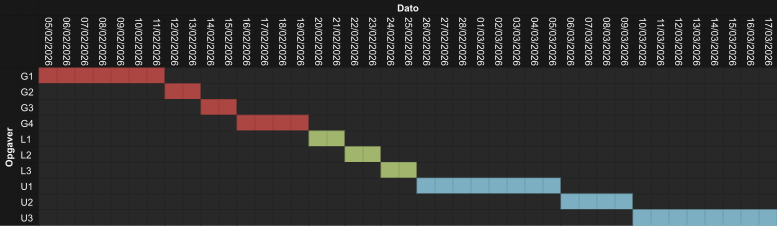
\includegraphics[width=1\textwidth]{tidsplan.png}
  \caption{Gantt-diagram}
\end{figure}

\section{Metodologi}
Dette afsnit beskriver de enkelte delelementer af systemet og de udfordringer, 
der opstod under implementeringsprocessen. Formålet er at give et klart overblik 
over, hvordan systemet blev udviklet, hvilke teknologier der blev anvendt, og 
hvordan forskellige funktionelle dele blev integreret.

\subsection{Brugergrænseflade}
Layoutsystemet MicroUI blev benyttet, da det bygger på renderingsfilosofien
immediate-mode. Dette gør det nemt at tegne, da alle grafiske elementer
gentegnes på hver frame, uden at det er nødvendigt at vedligeholde komplekse
graftræer af grafiske elementer. 

Der har været tvivl om, hvorvidt immediate-mode layoutsystemer kræver 
betydeligt mere strøm end traditionelle retained-mode layoutsystemer. Målinger 
viser dog, at dette ikke er tilfældet: under typiske forhold er energiforbruget 
for immediate-mode layoutsystemer sammenligneligt med, eller lavere end,
retained-mode layoutsystemer~\cite{smith2024_proving}. 
Dette indikerer, at frygten for øget strømforbrug ikke bør være en hindring
for at vælge immediate-mode layoutsystemer, og at valget i stedet kan baseres på
udviklingsmæssige og arkitektoniske fordele, såsom enkel genopbygning af den
grafiske flade og mindre kompleksitet.

Det ovenstående system fokuserer udelukkende på layoutet,
mens hele renderingsprocessen er håndskrevet i OpenGL ES 3.0 for at sikre optimal ydeevne.
Grafikrendering opnås ved hjælp af skræddersyet shader-kode,
der effektivt kan tegne rektangler. Disse rektangler udgør en fundamental byggesten i de
fleste grafiske brugergrænseflader (se \ref{lst:renderer}).

\begin{lstlisting}[language=C, caption=Vertex og Fragment shader, label=lst:renderer]
  static const char* vertex_shader_source = R"(#version 300 es
  precision mediump float;

  layout (location = 0) in vec2 a_position;
  layout (location = 1) in vec2 a_size;
  layout (location = 2) in vec2 a_center_coordinates;
  layout (location = 3) in vec2 a_texture_coordinates;
  layout (location = 4) in vec4 a_color;
  layout (location = 5) in float a_border_radius;

  uniform mat4 u_projection;

  out vec2 size;
  out vec2 center_coordinates;
  out vec2 texture_coordinates;
  out vec4 color;
  out float border_radius;

  void main()
  {
    gl_Position = u_projection * vec4(a_position, 0.0, 1.0);

    size = a_size;
    center_coordinates = a_center_coordinates;
    texture_coordinates = a_texture_coordinates;
    color = a_color;
    border_radius = a_border_radius;
  }
  )";

  static const char* fragment_shader_source = R"(#version 300 es
  precision mediump float;

  in vec2 size;
  in vec2 center_coordinates;
  in vec2 texture_coordinates;
  in vec4 color;
  in float border_radius;
  
  uniform sampler2D u_texture;
  
  out vec4 o_color;

  void main()
  {
    float relative_border_radius = border_radius * min(size.x, size.y);
    float distance = length(max(abs(gl_FragCoord.xy - center_coordinates) -
    size / 2.0f + relative_border_radius, 0.0)) - relative_border_radius;

    if (distance <= 0.0) {
      float anti_aliasing = fwidth(distance);
      float alpha = 1.0 - smoothstep(0.0, anti_aliasing, distance);
      alpha *= texture(u_texture, texture_coordinates).r;
      o_color = vec4(color.rgb, color.a * alpha);
    } else {
      o_color = vec4(0.0, 0.0, 0.0, 0.0);
    }
  } 
  )"; 
\end{lstlisting}

\subsection{Databehandling}
Der benyttes en skræddersyet hukommelsesallokator, da den standard hukommelsesallokator,
malloc/free, fungerer som et synkront håndtag, der hurtigt kan føre til komplekse allokeringsmønstre og
dermed betragtes som usikker. I stedet anvendes en kombination af arena- og stack-allokatorer.

Arena-allokatoren muliggør effektiv håndtering af noter i hukommelsen,
da allokeringen sker i en lineær buffer. Dette skaber en overskuelig mental model over den allokerede hukommelse og
gør det nemt at allokere eller frigive dele af bufferen samt hele bufferen (se \ref{fig:arena-allocate}).

\begin{figure}[h]
  \centering
  \includegraphics[width=1\textwidth]{arena-allokering.png}
  \caption{Arena allokering}
  \label{fig:arena-allocate}
  \centering
\end{figure}

Stack-allokatoren muliggør hurtig navigation frem og tilbage i brugergrænsefladen, idet den bygger på
Last In, First Out (LIFO)-princippet. Denne tilgang minimerer risikoen for hukommelsesfejl og skaber samtidig en
overskuelig mental model over den allokerede hukommelse (se \ref{fig:stack-allocate}).

\begin{figure}[h]
  \centering
  \includegraphics[width=1\textwidth]{stack-allokering.png}
  \caption{Stack allokering}
  \label{fig:stack-allocate}
  \centering
\end{figure}

\subsection{Datalagring}
Der benyttes en relationel database, mere specifikt en SQL database som datalagrings løsning.
Formålet med at anvende en relationel database er at skabe meningsfulde relationer mellem de
decentrale enheder og noterne. Ved at organisere data i tabeller kan vi effektivt håndtere og
forespørge de forbindelser, der eksisterer mellem forskellige enheder og deres tilknyttede noter.
SQL giver desuden mulighed for at køre komplekse forespørgsler, hvilket gør det lettere at opdatere,
søge og analysere informationen. Denne struktur bidrager til et mere strømlinet og effektivt system,
som kan skalere, efterhånden som der tilføjes flere enheder og noter (se \ref{fig:er-diagram}).

\begin{figure}[h]
  \centering
  \includegraphics[width=1\textwidth]{er-diagram.png}
  \caption{ER-diagram}
  \label{fig:er-diagram}
  \centering
\end{figure}

\section{Begrænsninger}

\section{Realiseret tidsplan}

\section{Konklusion}

\printbibliography[title={Referencer}]

\end{document}
